\documentclass{article}
\textheight 23.5cm \textwidth 15.8cm
%\leftskip -1cm
\topmargin -1.5cm \oddsidemargin 0.3cm \evensidemargin -0.3cm
%\documentclass[final]{siamltex}

\usepackage{ctex}
\usepackage{verbatim}
\usepackage{fancyhdr}
\usepackage{graphicx}
\usepackage{amsmath}
\usepackage{amssymb}
\usepackage{float}
\usepackage{multirow}
\usepackage{colortbl}
\usepackage{amsthm}
\usepackage{bm}
\usepackage{tikz}

\textheight 23.5cm \textwidth 15.8cm
\topmargin -1.5cm \oddsidemargin 0.3cm \evensidemargin -0.3cm
\title{HW3 实验报告}
\author{PB20010429 侯相龙}

\begin{document}
\maketitle
\section{实验内容}
实现泊松融合算法。具体来说,是将一张图像中的一个区域(ROI)融合到另一张图像中的指定位置,
使得融合后的图像看起来自然、连续。

\section{实验原理}

将背景图的部分区域赋予新的值,并要求其不仅满足前景图ROI的部分性质,也满足背景图的部分性质,已达到
自然连续的融合效果。具体来说,求解
\[\underset{f}{\operatorname{argmin}} \iint_{\Omega}|\nabla f-\nabla I|^{2}, \quad \text { s.t. } \quad f=g \quad \text { on } \partial \Omega\]
其中,I为前景图ROI的取值,g为背景图ROI的取值.

由变分法中的Euler-Lagrange Equation ,上述问题转化问求解
\[\Delta f=\Delta I \quad \text { in } \Omega, \quad \text { s.t. } \quad f=g \quad \text { on } \partial \Omega\]

在图像处理中,我们考虑离散的拉普拉斯方程(二阶差分形式)。并将ROI中邻居(上下左右)均属于ROI的点作为内点,反之作为边界点。
\section{算法介绍与步骤}
\begin{description}
    \item[1)]将输入的两张图像(背景图像和前景图像)都转换为 double 类型,并将像素值缩放到 [0,1] 范围内。
    \item[2)]将 ROI 区域的掩模图像应用到源图像和目标图像上,提取出 ROI 区域,并建立对应的线性索引,以待后续建立泊松方程
    \item[3)]按照原理中的方法将ROI区域分为内点和边界点。
    \item[4)]寻找内点邻居的线性索引,边界点的线性索引。并通过此建立系数矩阵。
    \item[5)]Laplace核作用于前景图像ROI和计算背景边界得到方程右端项,并解稀疏方程组。
    \item[6)] 最后将融合图像的像素值转换为 uint8 类型,即可输出融合结果。
\end{description}


\section{测试数据与实验结果}

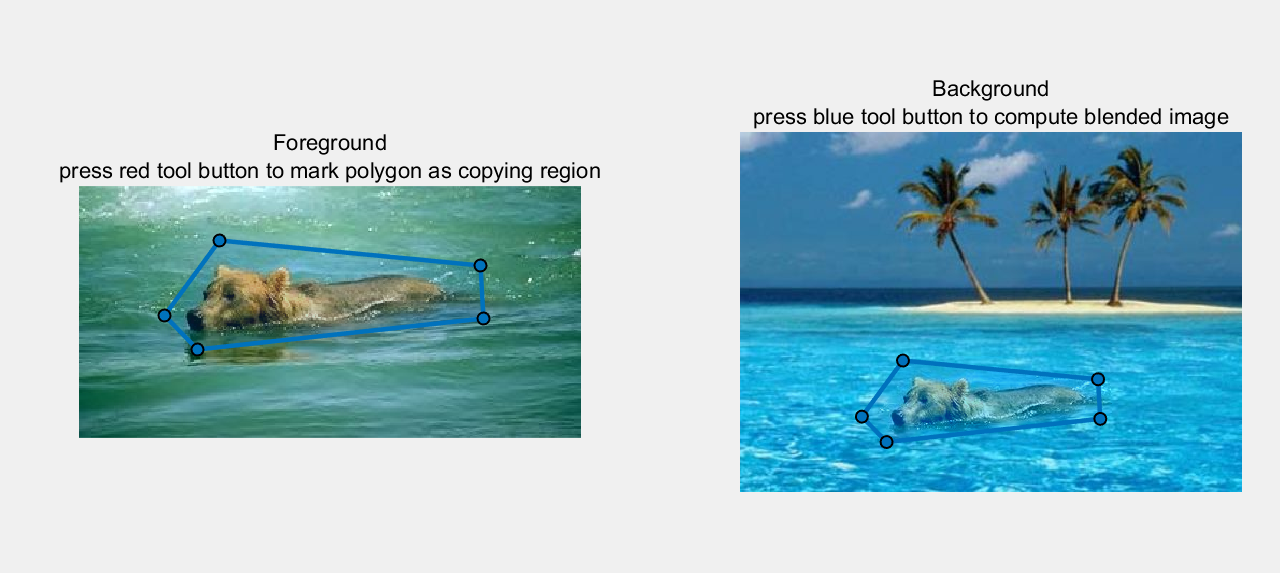
\includegraphics[width=0.8\textwidth]{1}

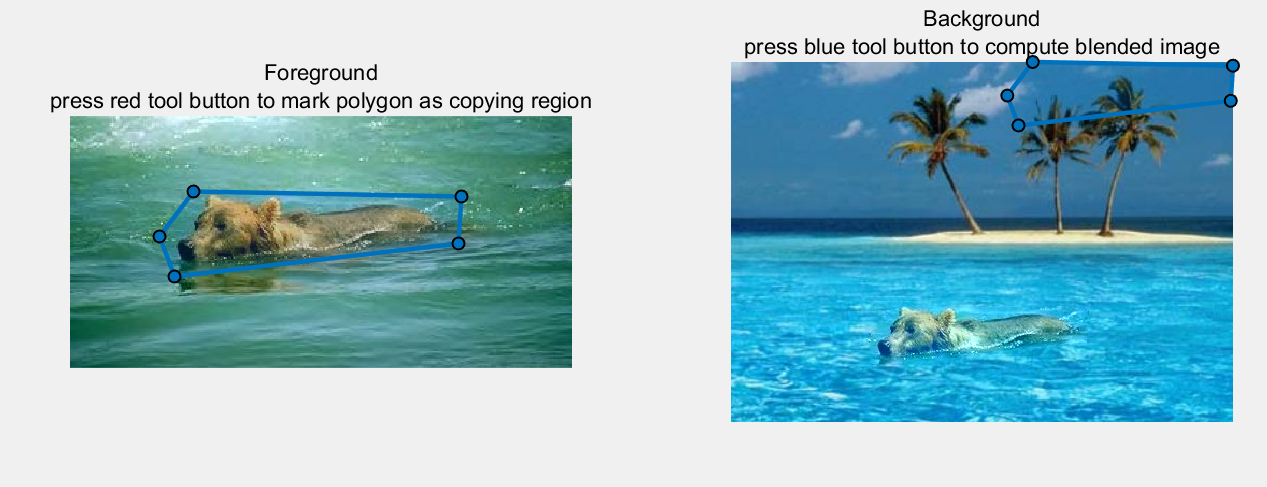
\includegraphics[width=0.8\textwidth]{2}

\section{实验总结}

本实验中,最大的难点在于向量化处理。
通过向量化,程序只有对通道的三次循环(可以忽略),没有对点的循环,实现的效率很高。

\end{document}
